\subsection{Dữ liệu đồ thị}
Trong thực tế, có rất nhiều bài toán có thể đưa về dạng đồ thị như bài toán liên quan đến phân tử hóa học, mạng xã hội, ... Ta có thể hiểu đồ thị là một hệ thống của các mối liên hệ và sự tương tác - điều này được thể hiện rõ nhất ở cạnh giữa hai đỉnh trong một đồ thị. Để tường minh hơn, Hình \ref{fig:vdgraph} sẽ cho một ví dụ cụ thể hơn:

\begin{figure}[H]
    \centering
    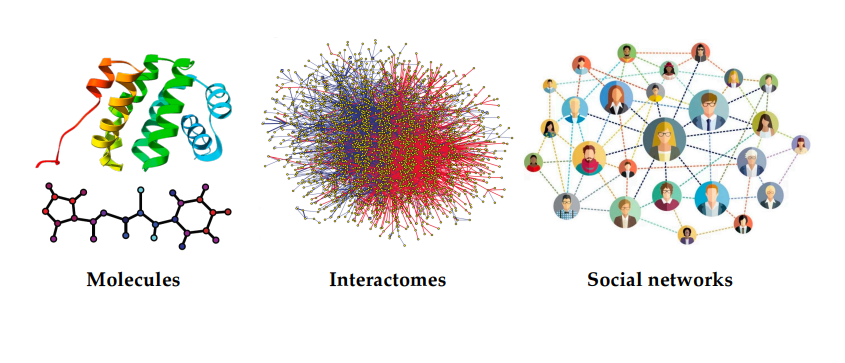
\includegraphics[width=0.7\linewidth]{Images/GDL/graph/graph_vd.png}
    \caption{Ví dụ minh họa về biểu diễn đồ thị của một số dữ liệu thực thế\cite{geometricdeep2022}}
    \label{fig:vdgraph}
\end{figure}

Tuy nhiên, ngoài tập các đỉnh và tập các cạnh của đồ thị ra thì trong mạng nơ-ron đồ thị (GNN) còn thêm một biểu diễn nữa là đặc trưng của các đỉnh. Các đặc trưng này sẽ thể hiện tính chất của các đỉnh ví dụ như đối với mạng xã hội thì là tuổi tác, số lượng bạn bè, ...

\begin{figure}[H]
    \centering
    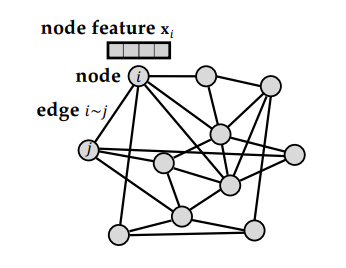
\includegraphics[width=0.7\linewidth]{Images/GDL/graph/graph_represent.png}
    \caption{Minh họa dữ liệu đồ thị trong GNN\cite{geometricdeep2022}}
\end{figure}

Trong GNN, ta có thể đánh số thứ tự các đỉnh tùy ý mà không làm thay đổi cấu trúc của đồ thị, do đó ta cần thiết kết một hàm có đầu vào là đặc trưng các đỉnh và ma trận kề sao cho nó phải bất biến với phép đánh thứ tự các đỉnh. Hay nói cách khác, hàm này phải là một hàm \textit{invariant permutation}. Điều này sẽ giúp cho đặc trưng của các đỉnh sau khi được tổng hợp không bị thay đổi khi ta đánh lại thứ tự các đỉnh.

Tuy nhiên, mặc dù hàm tổng hợp đặc trưng của các đỉnh là bất biến với phép hoán vị nhưng thứ tự các đặc trưng sau khi bị hoán vị vẫn phải thay đổi. Cụ thể hơn, nếu như thứ tự đặc trưng đầu vào bị thay đổi thì thứ tự đặc trưng sau khi tổng hợp đặc trưng cho các đỉnh cũng phải thay đổi, ví dụ: đồ thị có 3 đỉnh thì ta đánh thứ tự là 1, 2, 3 tuy nhiên khi ta hoán vị vị trí các đỉnh là 2, 1, 3 thì sau khi tổng hợp đặc trưng thì thứ tự cũng phải là 2, 1, 3 chứ không phải là 1, 2, 3. Điều này thể hiện tính \textit{equivariant} của GNN.

\begin{figure}[H]
    \centering
    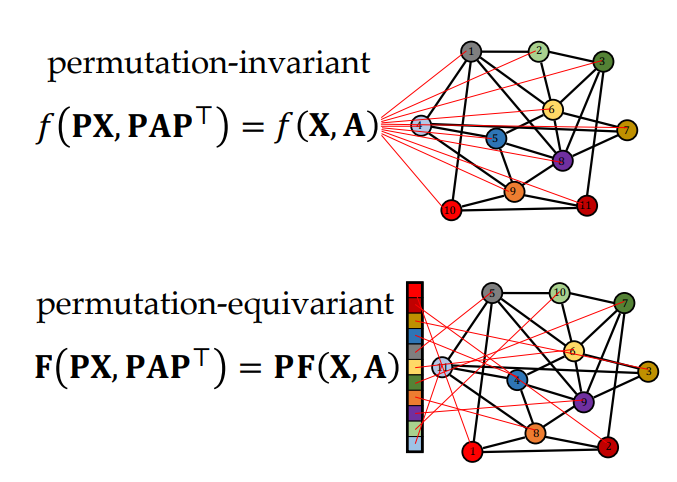
\includegraphics[width=1\linewidth]{Images/GDL/graph/inva_equi_permutation.png}
    \caption{Ảnh minh họa về \textit{invariant} và \textit{equivariant} trong GNN\cite{geometricdeep2022}}
\end{figure}

\begin{figure}[H]
    \centering
    \captionsetup{justification=centering}
    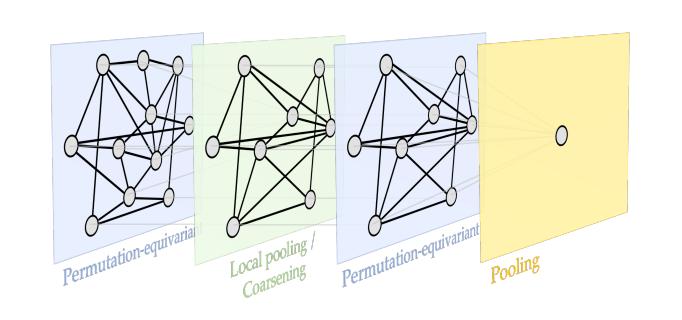
\includegraphics[width=1\linewidth]{Images/GDL/graph/gnn_structure.png}
    \caption{Cấu trúc của một mạng GNN, trong đó pooling là phép ánh xạ đưa một đồ thị thành một vector\cite{geometricdeep2022}}
\end{figure}

\vspace{-0.5cm}

Tiếp theo, báo cáo sẽ đưa ra cấu trúc của một hàm tổng hợp đặc trưng cho một đỉnh trong GNN. Ý tưởng trung của GNN là đặc trưng của một đỉnh sẽ bị ảnh hưởng bởi những đỉnh lân cân và chính nó. Do đó, các cấu trúc GNN khác nhau chỉ là các cách tổng hợp đặc trưng khác nhau và chúng được gọi chung bằng một cái tên là \textit{"message passing"}. 
\begin{figure}[H]
    \centering
    \captionsetup{justification=centering}
    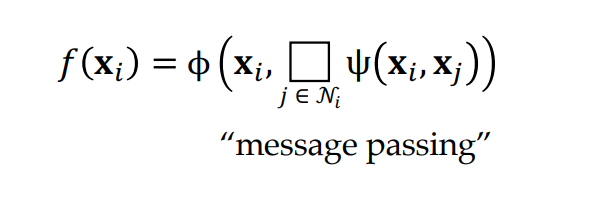
\includegraphics[width=0.7\linewidth]{Images/GDL/graph/message_passing.png}
    \caption{Cấu trúc của \textit{"message passing"} trong GNN, trong đó ô vuông là phép tổng hợp đặc trưng của các lân cận như là phép lấy tổng, trung bình, ...\cite{geometricdeep2022}}
\end{figure}

\vspace{-0.5cm}

Cụ thể hơn, báo cáo sẽ trình bày về hai ví dụ cụ thể của GNN là mạng nơ-ron tích chập (GCN) và mạng nơ-ron chú ý (GAT). Đầu tiên, đối với GCN thì ta chỉ lấy tổng các đặc trưng của lân cận nhân với một trọng số $c_{ij}$ thể hiện mức độ ảnh hưởng đến đỉnh của nó\cite{gcn_paper}. Tuy nhiên hệ số này lại không được tính thông qua bất kì biến nào mà chỉ là một tham số học thông thường. Dó đó, GAT \cite{gat_paper} đã thay thế trọng số $c_{ij}$ thành một hàm tính trọng số với đầu vào là hai đặc trưng của đỉnh hiện tại  $i$ và đỉnh lân cận $j$. Điều này sẽ giúp mô hình có được hệ số chính xác hơn về mức độ ảnh hưởng của các lân cận $j$ đến $i$.

\begin{figure}[H]
    \centering
    \captionsetup{justification=centering}
    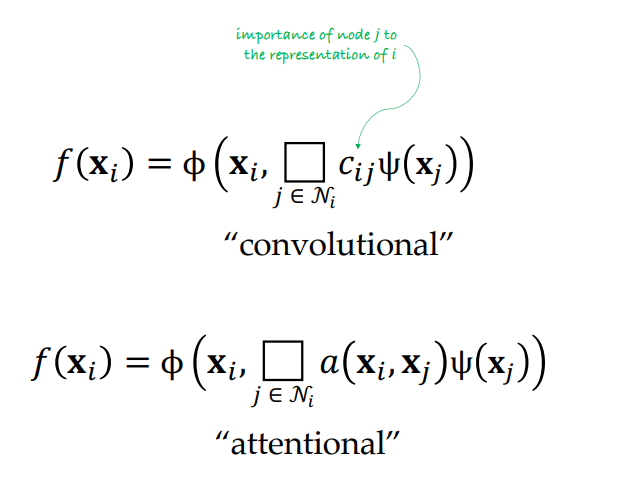
\includegraphics[width=0.7\linewidth]{Images/GDL/graph/gcn_gat.png}
    \caption{Cấu trúc của hàm tổng hợp thông tin của GCN và GAT\cite{geometricdeep2022}}
\end{figure}

Mặc dù GNN thường được biết đến là mạng nơ-ron làm việc với dữ liệu dạng đồ thị nhưng thực tế, nó có một số dạng đặc biệt mà được gọi với tên gọi khác. Dưới đây là một số trường hợp đặc biệt của GNN:

\begin{itemize}
    \item DeepSets\cite{zaheer2018deepsets}: Đây là một mạng nơ-ron làm việc trên tập các điểm ví dụ như point cloud. Do đó, ta có thể coi mạng này là một GNN làm việc với đồ thị không có cạnh.

    \begin{figure}[H]
    \centering
    \captionsetup{justification=centering}
    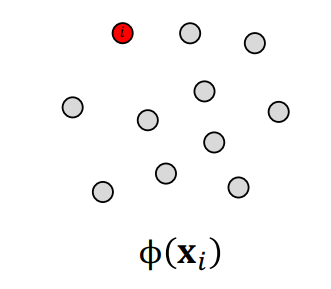
\includegraphics[width=0.4\linewidth]{Images/GDL/graph/deepset.png}
    \caption{Ảnh minh họa DeepSet\cite{geometricdeep2022}}
\end{figure}

    \item Transformers\cite{vaswani2023attentionneed}: Đây là một kiến trúc mạng nơ-ron rất nổi tiếng trong xử lý ngôn ngữ tự nhiên (NLP). Transformers tính hệ số attentions từ một từ đến tất cả các từ khác trong câu. Do đó, nếu ta coi các từ này là một đỉnh của đồ thị và trọng số attention chính là các cạnh thì đây chính là một đồ thị đầy đủ, cho nên, có thể coi Transformers là một mạng GNN làm việc trên đồ thị đầy đủ.

    \begin{figure}[H]
    \centering
    \captionsetup{justification=centering}
    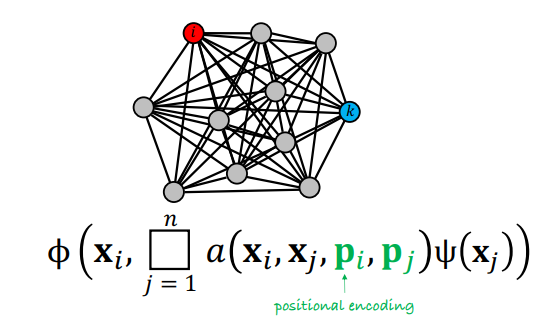
\includegraphics[width=0.7\linewidth]{Images/GDL/graph/transformer.png}
    \caption{Ảnh minh họa Transformer\cite{geometricdeep2022}}
\end{figure}

\end{itemize}

Thông thường đồ thị mà chúng ta làm việc với GNN là chỉ có đặc trưng của các đỉnh mà chưa hề có tọa độ của các đỉnh, ví dụ như đồ thị biểu diễn của một chất hóa học. Do đó, nếu ta làm việc với đồ thị được nhúng vào trong một không gian Euclid, ngoài việc các hàm phải \textit{invariant} và \textit{equivarint} đối với phép hoán vị chỉ số, ta sẽ cần phải thiết kế các hàm \textit{invariant} và \textit{equivarint} đối với các tác động của nhóm phép quay, nghịch đảo, dịch chuyển, phản chiếu\cite{geometricdeep2022}.

\begin{figure}[H]
    \centering
    \captionsetup{justification=centering}
    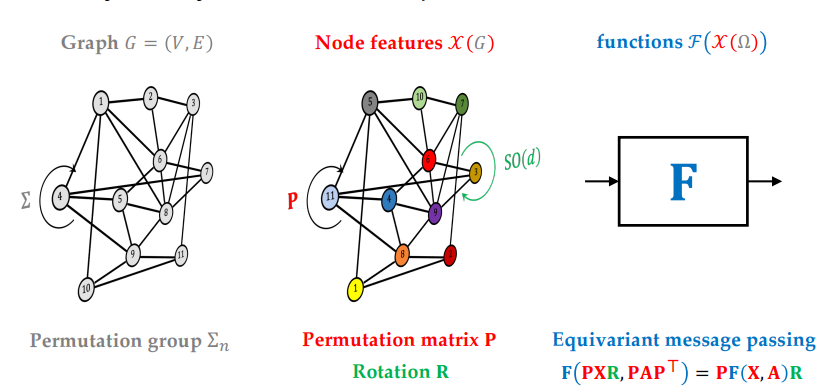
\includegraphics[width=1\linewidth]{Images/GDL/graph/gnn_geometric.png}
    \caption{Ảnh minh họa dữ liệu đồ thị hình học và các phép toán đại số tác động nên nó\cite{geometricdeep2022}}
\end{figure}


\subsection{Dữ liệu đa tạp}
Đa tạp\cite{wikipedia-datap} bản chất là một cấu trúc hình học mà trong đó cục bộ là một không gian Euclid. Ví dụ đơn giản nhất chính là trái đất mà chúng ta đang sống, ta đều biết rằng trái đất có cấu trúc hình học là hình cầu tuy nhiên nếu nhìn cục bộ trên trái đất thì lại là một mặt phẳng (giống như những gì chúng ta nhìn thấy khi đang đứng trên trái đất).

Mặc dù đa tạp có cấu trúc phức tạp nhưng nó lại có tính chất rất quan trong là lân cận. Do đó, để có thể sử dụng các phương pháp học máy để xử lý dạng dữ liệu này thì ta hoàn toàn có thể biểu diễn nó dưới dạng đồ thị, từ đó ta có thể nhúng nó vào một không gian rồi tính toán trên không gian này\cite{geometricdeep2022}. Tuy nhiên đây là cách khá là lâu đời, do đó, ta có thể thực hiện một cách khác là sử dụng GNN lên đồ thị mà không cần phải nhúng đồ thị này vào một không gian nào đó\cite{geometricdeep2022}.

\begin{figure}[H]
    \centering
    \captionsetup{justification=centering}
    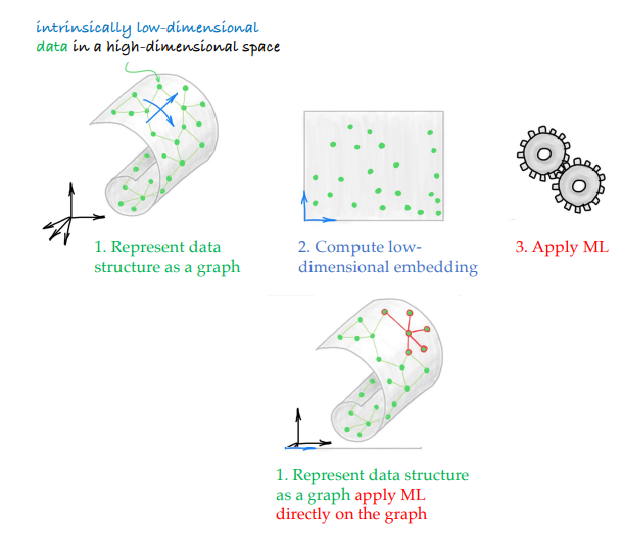
\includegraphics[width=0.7\linewidth]{Images/GDL/graph/manifold.png}
    \caption{Ảnh minh họa hai phương pháp trong \textit{manifold learning}\cite{geometricdeep2022}}
\end{figure}

\subsection{Dữ liệu dạng grid}
Ta có thể coi \textit{grid} là một đồ thị vành (\textit{ring graph})\cite{geometricdeep2022}. Dữ liệu ở dạng này thì các đỉnh sẽ bị cố định cấu trúc lân cận và do đó, ta chỉ cần định nghĩa một hàm tổng hợp đặc trưng cho mỗi đỉnh khá là đơn giản. Hình \ref{fig:grid_ex} là một ví dụ minh họa về \textit{grid}:

\begin{figure}[H]
    \centering
    \captionsetup{justification=centering}
    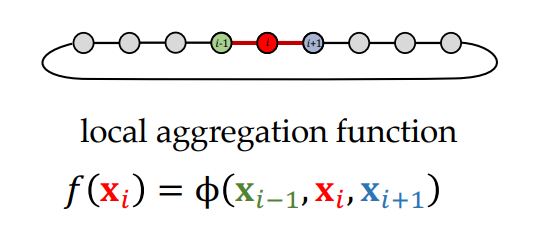
\includegraphics[width=0.7\linewidth]{Images/GDL/graph/grid_ex.png}
    \caption{Ảnh minh họa dữ liệu dạng \textit{grid} và cấu trúc hàm tổng hợp đặc trưng\cite{geometricdeep2022}}
    \label{fig:grid_ex}
\end{figure}

Như ta có thể thấy trong hình \ref{fig:grid_ex} thì hàm tổng hợp đặc trưng chỉ đơn giản là một hàm nhận vào 3 tham số mà không cần đưa input vào một hàm nào khác như GNN. Để tổng quát hơn, ta có thể coi hàm này là tổ hợp tuyến tính của ba tham số đầu vào: $f(x_i) = a x_{i-1} + b x_{i} + c x_{i+1}$ \cite{geometricdeep2022}

\begin{figure}[H]
    \centering
    \captionsetup{justification=centering}
    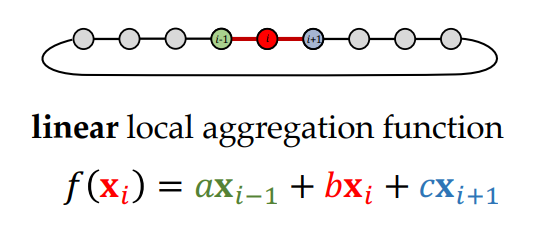
\includegraphics[width=0.7\linewidth]{Images/GDL/graph/grid_agg.png}
    \caption{Ảnh minh họa hàm tổng hợp đặc trưng đối với dữ liệu \textit{grid}\cite{geometricdeep2022}}
\end{figure}


